\documentclass[eikonal.tex]{subfiles}

\begin{document}

\section{Implementation of the ordered line integral
  method}\label{sec:implementation}

In this section, we describe how to implement \cref{enum:update-U} of
\cref{alg:dijkstra-like} efficiently.

\subsection{Simplex selection}

Computing $U(\hat{p})$ consists of determining a set of possible
directions for the first arrival characteristic and then solving a
sequence of optimization problems to find it. In 2D, we consider two
types of neighborhoods: neighborhoods where $p \in \neib(\hat{p})$ is
such that $\hat{p} - p$ has at most one nonzero component or at most
two nonzero components (recalling that we always assume
$\norm{p}_\infty \leq 1$ for $p \in \mathbb{Z}^n$). The former is the
$\ell_1$ neighborhood of $\hat{p}$, the latter is the $\ell_\infty$
neighborhood. In 3D, we also consider the $\ell_1$ and $\ell_\infty$
neighborhood, corresponding to a 6-point and 26-point neighborhood,
respectively. We also consider an 18-point neighborhood, consisting of
$p$ such that $\hat{p} - p$ has at most two nonzero components.

With $\neib(\hat{p})$ defined, it becomes necessary determine which
simplices are candidates for optimization. One natural approach would
be to discretize the surface of the convex hull of the neighborhood of
points into triangles (e.g., in 3D) and let the set of admissible
triangles and tetrahedra be the convex hulls of the lines and
triangles lying on this discretizing surfaces and $\hat{p}$. For the
6-point, 18-point, and 26-point neighborhoods, these surfaces are an
octahedron, cuboctahedron, and cube, respectively. There are several
ways of decomposing these surfaces into triangle meshes.

Another approach is to assume that the simplices within each orthant
are the same. Then, we can restrict our attention to a single orthant
and determine the admissible simplices by selecting vertices. We would
like these simplices to be symmetric about the diagonal of the orthant
so that our update is isotropic. Following this idea, we decompose an
octant into groups of tetrahedra in
\cref{fig:octant-numbering,fig:olim18-tetrahedra,fig:olim26-tetrahedra}
in \cref{sec:tetra-groups}. We partially sort the vertices of octant
by degree, allowing us to easily separate our groups into groups which
features in the 6-point, 18-point, or 26-point neighborhoods.

\subsection[Optimization algorithms]{Optimization algorithms for the
  constrained problem}

In this section, we describe two optimization algorithms for solving
the constrained minimization problem
\cref{eq:constrained-minimization}. To compute $U(\hat{p})$ in
\cref{alg:dijkstra-like}'s \cref{enum:update-U}, multiple instances of
\cref{eq:constrained-minimization} with overlapping boundaries must be
solved. The fact that the boundaries of their domains overlap leads to
different algorithms for solving all instances of
\cref{eq:constrained-minimization} in tandem. This is discussed in the
next section.

For the following two algorithms, we assume that $F_i$ is strictly
convex. This is always the case for $F_0$, and holds for $F_1$ if $h$
is small enough.

Our first algorithm is a projected Newton's method. Variations of this
algorithm can be found in many sources,
e.g.~\cite{bertsekas1999nonlinear,nocedal2006numerical}. Minimizing
$F_i(\lambda)$, if we let $\lambda_k$ ($k = 0, 1, \hdots$) be a
sequence of iterates and
$\lambda_{k+1} = \lambda_k + \delta\lambda_k$, we can
Taylor expand:
\begin{equation}
  F_i(\lambda_k + \delta\lambda_k) = F_i(\lambda_k) + \nabla F_i(\lambda_k)^\top \delta\lambda_k + \frac{1}{2} \delta\lambda_k^\top \nabla^2 F_i(\lambda_k) \delta\lambda_k + O(\norm{\delta\lambda_k}^3).
\end{equation}
A common approach to minimizing nonlinear functions is minimizing a
sequence of local quadratic approximations. If our goal is to minimize
$F_i(\lambda_{k+1})$, we find an approximate optimum by instead
solving:
\begin{equation}\label{eq:local-quadratic-minimization}
  \begin{split}
    \min_{\lambda} &\qquad \frac{1}{2} \lambda^\top \nabla^2 F_i(\lambda_k) \lambda + \nabla F_i(\lambda_k)^\top \lambda \\
    \text{subject to} &\qquad \lambda \in \Delta^d.
  \end{split}
\end{equation}
\Cref{eq:local-quadratic-minimization} is an inequality constrained
quadratic program (IQP) which can be solved using the active set
method~\cite{nocedal2006numerical}, the details of which are outside
the scope of this paper. One thing to note is that the constraints
encapsulated by $\lambda \in \Delta^d$ can be written in matrix form
(e.g., for $d = n$) as:
\begin{equation}
  \label{eq:matrix-ineq}
  A \lambda \geq b, \qquad \text{where} \qquad A = \begin{bmatrix}
    -\m{1}_{1 \times n} \\ I_n
  \end{bmatrix}, \qquad b = \begin{bmatrix} -1 \\ \m{0}_{n \times 1} \end{bmatrix}.
\end{equation}
The simplicity of \cref{eq:matrix-ineq} makes the implementation of
the active set method for solving
\cref{eq:local-quadratic-minimization} simpler and more efficient.

\begin{algorithm}[H]
  \caption{Projected Newton's method for solving
    \cref{eq:constrained-minimization} with
    $F_i^\theta = F_1^\theta$.}\label{alg:proj-newton}
  \begin{enumerate}[nolistsep]
  \item Initialize $\lambda_0$. We take $\lambda_0$ to be the centroid
    of $\Delta^n$.
  \item For $k = 1, 2, \hdots$ until convergence:
    \begin{enumerate}
    \item Set $H_k = \nabla^2 F_1^\theta(\lambda_k)$.
    \item Perturb $H_k$ by a small multiple of $I$ if $H_k$ isn't
      positive definite (optional, depending on $h$).
    \item Set $g_k = \nabla F_1^\theta(\lambda_k) - H_k \lambda_k$.
    \item Compute $p_k = \delta \lambda_k$ by solving
      $p_k = \argmin_{Ap \geq b - A\lambda_k} p^\top H_k p + g_k^\top
      p$ using the active set method.
    \item Compute a step size $\gamma_k$ using line search.
    \item Let $\lambda_{k + 1} = \lambda_k + \gamma_k p_k$.
    \end{enumerate}
  \item Compute $\hat{U}$ from the final $\lambda_k$.
  \end{enumerate}
\end{algorithm}

Using \cref{theorem:mp0-newton,thm:f0-exact}, we can avoid the use
of an algorithm for constrained optimized by first computing
$\lambda_0^*$ using \cref{thm:f0-exact} and then setting
$\lambda_0 = \lambda_0^*$ in an unconstrained Newton iteration
minimizing $F_1$. \Cref{theorem:mp0-newton,thm:f0-exact} give us
conditions for determing when this be done: in particular, we first
check if $\norm{R^{-\top} \delta U} < s^\theta h$, then check if
$\lambda_1^*$ inside $\Delta^n$. If this isn't the case, we can
default to \cref{alg:proj-newton}. \hl{\textbf{TODO}}: \emph{use
  $\lambda_0^*$ to initialize the projected Newton method when this
  happens.}

In the proof of \cref{theorem:mp0-newton}, $\lambda_1^*$ lies in the
closed ball $B_r(\lambda_0^*)$, where:
\begin{equation}
  r \leq R = \frac{\alpha}{1 - \alpha/2}, \mbox{ and } \alpha = \norm{\nabla^2 F_1(\lambda_0^*)^{-1} \nabla F_1(\lambda_0^*)}.
\end{equation}
Checking whether $\lambda_1^*$ is in $\Delta^n$ can then be done by
checking if $B_R(\lambda_0^*)$ is contained in $\Delta^n$.

\begin{algorithm}[H]
  \caption{Newton's method with warm start for solving
    \cref{eq:constrained-minimization} with
    $F_i = F_1$.}\label{alg:warm-start-newton}
  \begin{enumerate}[nolistsep]
  \item Compute the reduced QR decomposition $\delta P = QR$.
  \item Let $\lambda_0 = \lambda^*$ in \cref{eq:f0-exact-lambda}.
  \item If $B_R(\lambda_0) \subseteq \Delta^n$, then:
    \begin{enumerate}[nolistsep]
    \item For $k = 1, 2, \hdots$ until convergence:
      \begin{enumerate}
      \item Set
        $\lambda_k = \lambda_{k-1} - \nabla^2
        F_1(\lambda_{k-1})^{-1} \nabla
        F_1(\lambda_{k-1})$.
      \end{enumerate}
    \item Evaluate $\hat{U}$ using the last $\lambda_k$ iterate.
    \end{enumerate}
  \item Otherwise, run \cref{alg:proj-newton}.
  \end{enumerate}
\end{algorithm}

\subsection[Update algorithms]{Hierarchical update algorithms}

We can envision general $n$-dimensional eikonal solvers which involve
correspondingly more complicated complexes of update simplexes. As $n$
grows, to avoid an exponential increase in the amount of work required
to update a node, we adopt a hierarchical algorithm which reduces the
number of simplexes which need to be traversed. For any dimension $n$,
we start by computing the minimal degree 1 (line) update. We then
evaluate each degree 2 (triangle) update that contains the minimal
node just found. Likewise for degree 3 (tetrahedron) and higher. This
approach allows us to structure our search through a large set of
update simplexes intelligently. An added benefit is that this approach
allows us to take advantage of the Karush-Kuhn-Tucker (KKT) theory of
constrained optimization to skip higher degree updates based on our
knowledge of lower degree updates. This is described below. The
nascent idea that led to this algorithm was first developed to
accelerate a Dijkstra-like solver used to compute quasipotentials of
nongradient stochastic differential equations in
2D~\cite{dahiya2017ordered}.

\begin{equation}
  L_i(\lambda, \mu) = F_i(\lambda) + {(A\lambda - b)}^\top \mu.
\end{equation}

Since \cref{eq:constrained-minimization} only has linear inequality
constraints, and since we assume that $F_i$ is strictly convex
according to \cref{lemma:F-strictly-convex}, checking the KKT
conditions for \cref{eq:constrained-minimization} is
straightforward. If $(\lambda^*, \mu^*)$ satisfy:
\begin{equation}
  \label{eq:kkt}
  \begin{split}
    \nabla_\lambda L_i(\lambda^*, \mu^*) &= 0, \\
    A\lambda^* &\geq b, \\
    \mu^* &\geq 0, \\
    (A\lambda^* - b)^\top \mu^* &= 0,
  \end{split}
\end{equation}
then $\lambda^*$ is a global minimizer over $\Delta^n$.

Computing $\mu^*$ is easy. We can convert this into a simple and cheap
test for whether a simplex update is necessary to perform. For a given
argument $\lambda \in \Delta^n$, let $I$ be the set of active
constraints; i.e.:
\begin{equation}
  I = \set{i : (A\lambda)_i = b_i, \hspace{0.25em} 0 \leq i < n}.
\end{equation}
Also, let $A_I$ be a matrix consisting of the columns of $A$ indexed
by $I$, and let $\lambda_I$ and $b_I$ be subvectors of $\lambda$ and
$b$ indexed by $I$. The active set method used in
\cref{alg:proj-newton} solves equality-constrained quadratic programs
of the form:
\begin{equation}
  \label{eq:active-set-EQP}
  \begin{split}
    \min_{\delta \lambda} &\qquad \frac{1}{2} \delta \lambda^\top \nabla^2 F_i^\theta (\lambda) \delta \lambda + \nabla F_i^\theta(\lambda)^\top \delta \lambda \\
    \text{subject to} &\qquad A_I \delta \lambda = b_I - A_I \lambda,
  \end{split}
\end{equation}
to compute a candidate descent step $\delta \lambda$. The KKT system
corresponding to \cref{eq:active-set-EQP} is:
\begin{equation}
  \begin{bmatrix}
    \nabla^2 F_i (\lambda) & -A_I^\top \\
    A_I & 0
  \end{bmatrix} \begin{bmatrix}
    \delta\lambda^* \\ \mu
  \end{bmatrix} = \begin{bmatrix}
    -\nabla F_i(\lambda) \\ 0
  \end{bmatrix}.
\end{equation}
The vector of Lagrange multipliers can be computed from:
\begin{equation}
  \mu = {(A_I \nabla^2 F_i(\lambda)^{-1} A_I^\top)}^{-1} A_I \nabla^2 F_i(\lambda)^{-1} \nabla F(\lambda).
\end{equation}
If $\mu \geq 0$, then $\mu$ corresponds to the a global constrained
optimum over $\Delta^n$. We can use this to design a fast hierarchical
algorithm for computing $\hat{U}$.

\begin{algorithm}[H]
  \caption{A bottom-up hierarchical algorithm for computing
    $U(\hat{p})$ (\cref{enum:update-U} of
    \cref{alg:dijkstra-like}).}\label{alg:bottom-up}
  \begin{enumerate}[nolistsep]
  \item Find $p_0 \in \neib(\hat{p})$ such that $p_0$\texttt{.state}
    $=$ \texttt{valid} with the minimum update value for $d = 1$
    (\hl{\textbf{TODO}}: or do the parent node optimization...).
  \item For $i = 1, \hdots, n - 1$:
    \begin{enumerate}
    \item For each $p_i$ such that $p_i$\texttt{.state} $=$
      \texttt{valid} and $p_i \in$ \hl{\textbf{TODO}}:
      \begin{enumerate}
      \item Do the degree $d = i + 1$ update corresponding to
        $p_0, \hdots, p_{i-1}$ using \cref{alg:warm-start-newton}.
      \item Evaluate $\mu^*$ corresponding to $\lambda^*$ for the
        degree $d$ update. If $\mu^* \geq 0$, terminate our search and
        compute $\hat{U}$ using $\lambda^*$.
      \end{enumerate}
    \end{enumerate}
  \end{enumerate}
\end{algorithm}

In practice, \cref{alg:proj-newton} is converges rapidly and is
efficient in terms of its implementation.

\begin{figure}[t]
  \centering
  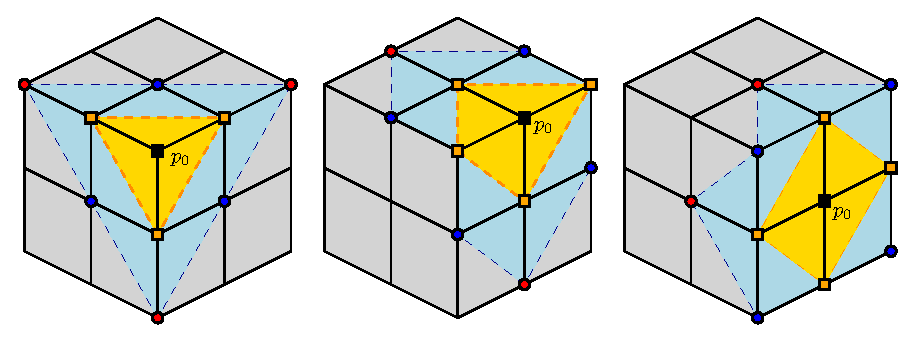
\includegraphics[width=0.85\linewidth]{hu-neighborhoods.eps}
  \caption{hi}
\end{figure}

Let $\calC_d$ be the set of degree $d$ update simplices for $\hat{p}$
such that each update vertex is \texttt{valid}. Since
\cref{alg:proj-newton} computes the constrained global optimum over an
update simplex, after running it, we can rule out any lower degree
incident update simplices. By starting with the highest degree update
simplices, we can progressively rule out large numbers of incident
subsimplices and substantially reduce the number of minimization
problems that need to be solved to compute each value $\hat{U}$.

\begin{algorithm}[H]
  \caption{A top-down hierarchical algorithm for computing
    $U(\hat{p})$ (\cref{enum:update-U} of
    \cref{alg:dijkstra-like}).}\label{alg:top-down}
  \begin{enumerate}[nolistsep]
  \item Let $\hat{U} = \infty$.
  \item For $d = n, n-1, \hdots, 1$:
    \begin{enumerate}
    \item For each $(p_0, \hdots, p_{d-1}) \in \calC_d$:
      \begin{enumerate}
      \item Compute $U$ for the update simplex
        $(p_0, \hdots, p_{d-1})$ using \cref{alg:proj-newton}.
      \item Set $\hat{U} = \min(\hat{U}, U)$.
      \item Remove each subsimplex consisting of choices of
        $p_0, \hdots, p_{d-1}$ from $\calC_1, \hdots, \calC_{d-1}$.
      \end{enumerate}
    \end{enumerate}
  \end{enumerate}
\end{algorithm}

\hl{\textbf{TODO}}

\subsection{Local factoring}

\hl{This section is messed up. Fix it.} In this section, we will
consider a single point source $x^\circ$, and let
$\boundary = \set{x^\circ}$. Let the grid
$\calG \subseteq \mathbb{Z}^n$ be aligned so that
$p^\circ \in \mathbb{Z}^n$. For a point $p_\lambda$, define
$l^\circ_\lambda = \norm{p_\lambda - p^\circ}$ and let
$s^\circ = s(x^\circ)$. Consider the additive factorization of $U$
around $x^\circ$:
\begin{align}
  U(x) = T(x) + \tau(x), \qquad \text{where} \qquad T(x) = s^\circ \norm{x - x^\circ},
\end{align}
i.e.\ $u_\lambda = T_\lambda + \tau_\lambda$ where
$T_\lambda = s^\circ h l^\circ_\lambda$. Our definition of
$F_i^\theta$ was such that $\hat{U} = F_i^\theta(\lambda^*)$. We will
define $G_i^\theta$ analogously. Note, e.g.\ for $i = 0$, that:
\begin{equation}
  \hat{\tau} = \hat{U} - \hat{T} = \tau_\lambda + T_\lambda - \hat{T} + s^\theta h l_\lambda,
\end{equation}
where $\tau_\lambda$ and $T_\lambda$ are defined analogously to
$U_\lambda$; i.e., $\tau_\lambda = \tau_0 + \delta \tau^\top \lambda$
and \hl{$T_\lambda = T_0 + \delta T^\top \lambda$} (\emph{pretty sure
  this is wrong and should be $T_\lambda = s^\circ l^\circ_\lambda$}),
where $\tau_i$ and $T_i$ are the values of $\tau$ and $T$ at $p_i$ for
each $i$. So, we define:
\begin{align}
  \label{eq:Gi}
  G_0^\theta(\lambda) &= \tau_\lambda + s^\circ h l^\circ_\lambda - s^\circ h \hat{l}^\circ + s^\theta h l_\lambda, \\
  G_1^\theta(\lambda) &= \tau_\lambda + s^\circ h l^\circ_\lambda - s^\circ h \hat{l}^\circ + s^\theta_\lambda h l_\lambda,
\end{align}
where $\hat{l}^\circ = \norm{\hat{p} - p^\circ} = \norm{p^\circ}$. As
for $F_0^\theta$ and $F_1^\theta$, the only difference between
$G_0^\theta$ and $G_1^\theta$ is between the terms containing
$s^\theta$ and $s^\theta_\lambda$.

\begin{figure}
  \centering
  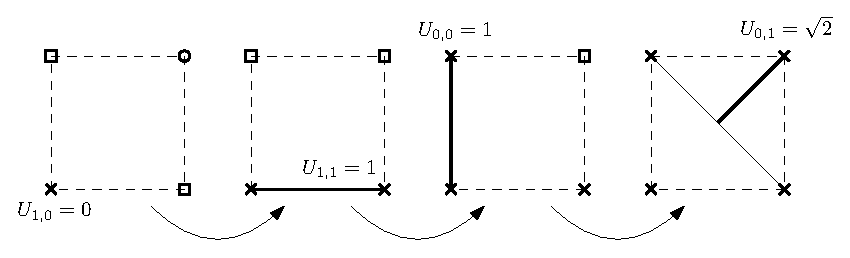
\includegraphics{factoring-example.eps}
  \caption{Factoring in action. This figure shows three steps of
    \texttt{olim4rhr} (or, equivalently, the four-point fast marching
    method with factoring). Ordered clockwise from the top left, the
    nodes are $p_{0, 0}, p_{0, 1}, p_{1, 1}$, and $p_{1, 0}$, with
    $h = 1$ (so we assume our domain is identified with
    $\mathbb{Z}^2$). We assume a constant slowness function:
    $s \equiv 1$. Initially, $p^\circ = p_{1, 0}$ is the only node in
    \texttt{bd} and is factored. The first two steps proceed exactly
    the same as for the unfactored method, since the steps between the
    source nodes and the updated nodes lie along characteristics of
    the solution, $u$. In the third step, the unfactored method would
    set $U_{0,1} \gets 1 + \nicefrac{\sqrt{2}}{2}$. For the factored
    method, since $\tau_{0,1} = 1 - 1 = 0 = \tau_{1,0}$, we find that
    $U_{0,1} \gets 0 + s^\circ l^\circ_{\nicefrac{1}{2}} + s^\theta h
    l_{\nicefrac{1}{2}} = \nicefrac{\sqrt{2}}{2} +
    \nicefrac{\sqrt{2}}{2} = \sqrt{2}$.}
\end{figure}

\begin{lemma}
  The gradient and Hessian of $G_i^\theta$ for $i = 0, 1$ are given
  by:
  \begin{align}
    \label{eq:G-grad-hess}
    \nabla G_i^\theta(\lambda) &= \nabla F_i^\theta(\lambda) + \frac{s^\circ h}{l^\circ_\lambda} \delta P^\top {(p_\lambda - p^\circ)} - \delta T, \mbox{(wrong)} \\
    \nabla^2 G_i^\theta(\lambda) &= \nabla^2 F_i^\theta(\lambda) + \frac{s^\circ h}{l^\circ_\lambda} \delta P^\top \calP^\perp_{p_\lambda - p^\circ} \delta P.
  \end{align}
\end{lemma}

\hl{\textbf{TODO}}: \emph{direct solution for $G_0^\theta$?}

\begin{figure}[h]
  \centering
  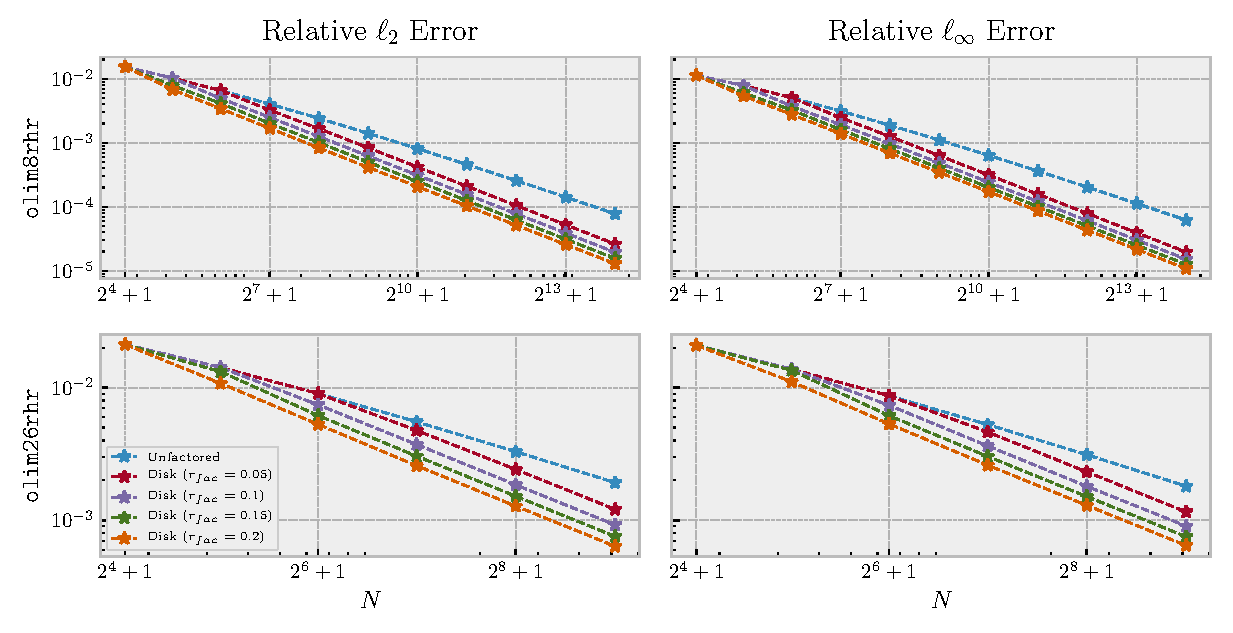
\includegraphics[width=\linewidth]{factoring-error-example.eps}
  \caption{\hl{TODO}}
  \label{fig:factoring-error-example}
\end{figure}

\end{document}

%%% Local Variables:
%%% mode: latex
%%% TeX-master: "sisc-eikonal.tex"
%%% End:
